\subsection{Quelques r�alisations (informatique)}

\frame{
  \frametitle{\insertsubsectionhead}
  %\frametitle{Quelques r�alisations (informatique)}

  \begin{itemize}

  \item Site web 

    %\vressort{1}

    \begin{center}
      \url{http://www.celles.net}
    \end{center}
    
    %\vressort{1}

    \begin{itemize}
    \item Site traitant de physique, d'informatique, d'�lectronique
    \item Site bas� sur le Wiki (Wikini)
    \item Am�lioration du moteur de Wikini (PHP), ajout de fonctionnalit�s
    \end{itemize}

  \end{itemize}

  %\vressort{1}

  \begin{center}
    \includegraphics[width=7cm]{site.eps}
  \end{center}

  %\vressort{1}
}

\frame{
  \frametitle{\insertsubsectionhead}

  \begin{itemize}
    
  \item fieldEB, simulateur d'�lectrostatique et de magn�tostatique

    \vressort{1}
  
    \begin{center}
      \url{http://www.celles.net/wikini/wakka.php?wiki=}\\
      \url{fieldEB}
    \end{center}
  \end{itemize}

  \vressort{1}

  \begin{center}
    \begin{tabularx}{\linewidth}{XX}
      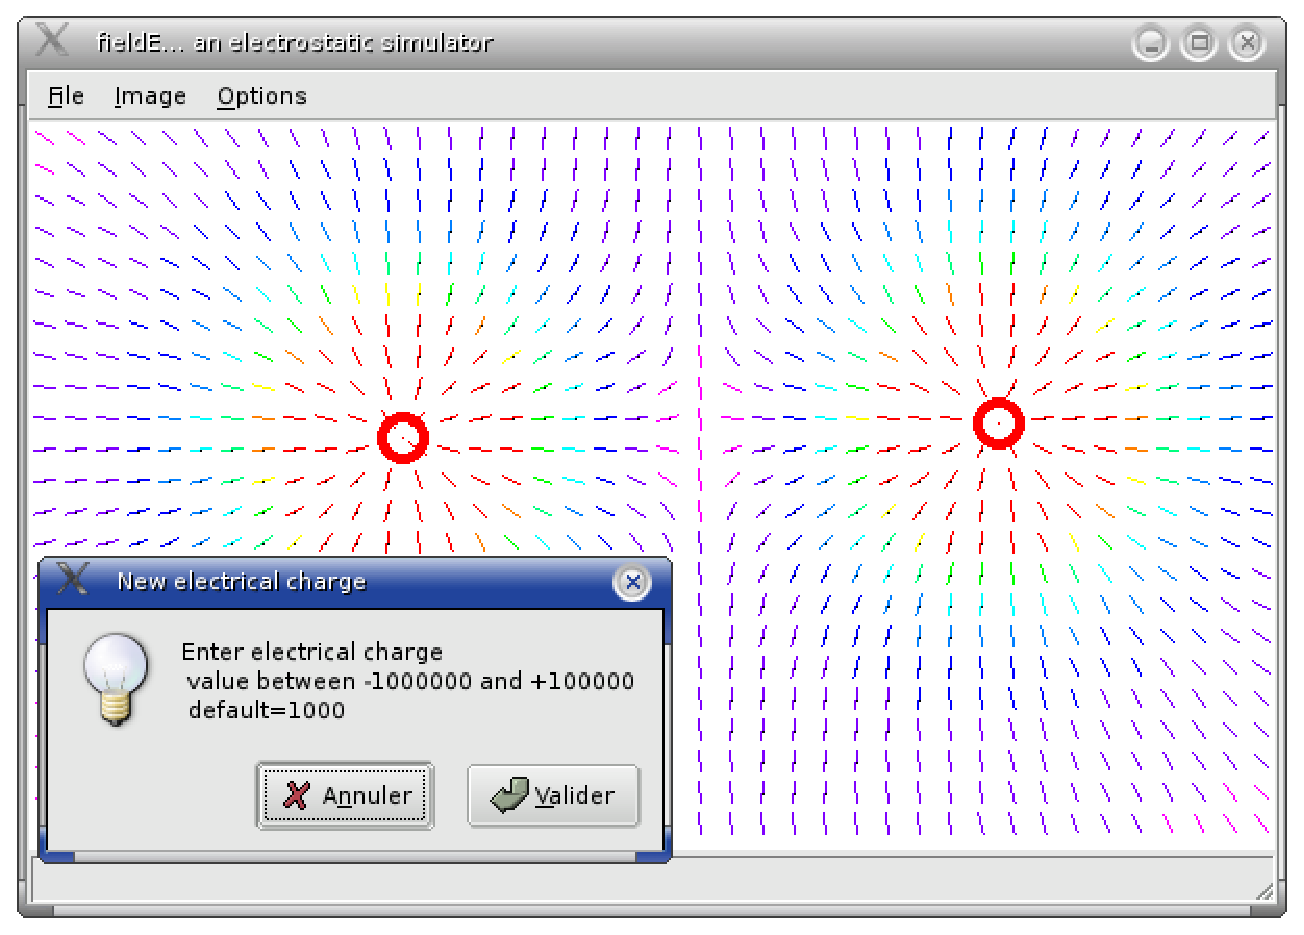
\includegraphics[width=4cm]{fieldeb_python_1.eps}
      &
      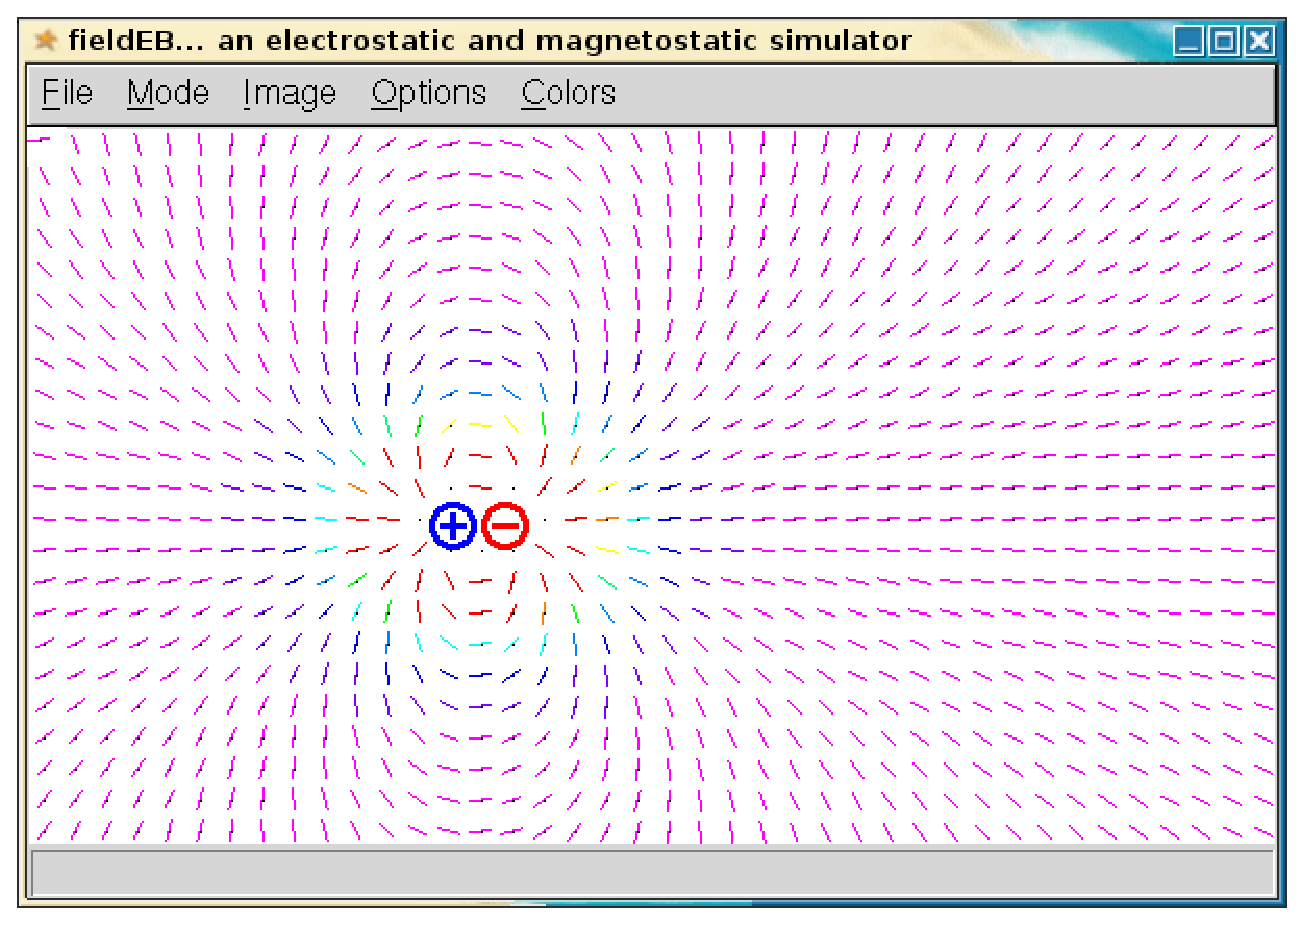
\includegraphics[width=4cm]{fieldeb_python_4.eps}
    \end{tabularx}
  \end{center}

  \vressort{1}
}

\frame{
  \frametitle{Quelques r�alisations (informatique)} 

  \vressort{1}   

  \begin{itemize}
  \item Harmon, recomposition de signaux � l'aide des harmoniques

    \vressort{1} 

    \begin{center}
      \url{http://www.celles.net/wikini/wakka.php?wiki=}\\
      \url{Harmon}
    \end{center}
    
    \vressort{1} 
    
  \end{itemize}

}

\frame{
  \frametitle{Quelques r�alisations (informatique)} 

  \begin{itemize}
  \item Divers exemples de calculs num�riques en Physique et en Math�matiques avec Scilab ou avec avec un simple tableur
    
    \begin{center}
      \url{http://www.celles.net/wikini/wakka.php?wiki=}\\
      \url{CalculNumerique}
    \end{center}

    \begin{itemize}
      \item M�canique
      \item Electrostatique / Magn�tostatique
      \item Automatique
      \item Electricit�
      \item Radioactivit�
      \item Son
      \item Traitement du signal
    \end{itemize}

  \end{itemize}
}

\frame{
  \frametitle{Quelques r�alisations (informatique)} 

  \begin{itemize}

  \item G�n�rateur en ligne de papiers sp�ciaux
    
    \begin{center}
      \url{http://www.celles.net/wikini/wakka.php?wiki=}\\
      \url{Papier}
    \end{center}

    \begin{itemize}
    \item \'Ecrit en PHP avec la biblioth�que FPDF pour g�n�rer des fichiers PDF
    \item D'autres papiers g�n�r�s avec \LaTeX\ et PSTricks sont �galement disponible
    \end{itemize}

  \end{itemize}
}

% \frame{
%   \begin{center}
%     \begin{tabularx}{\linewidth}{XX}
%       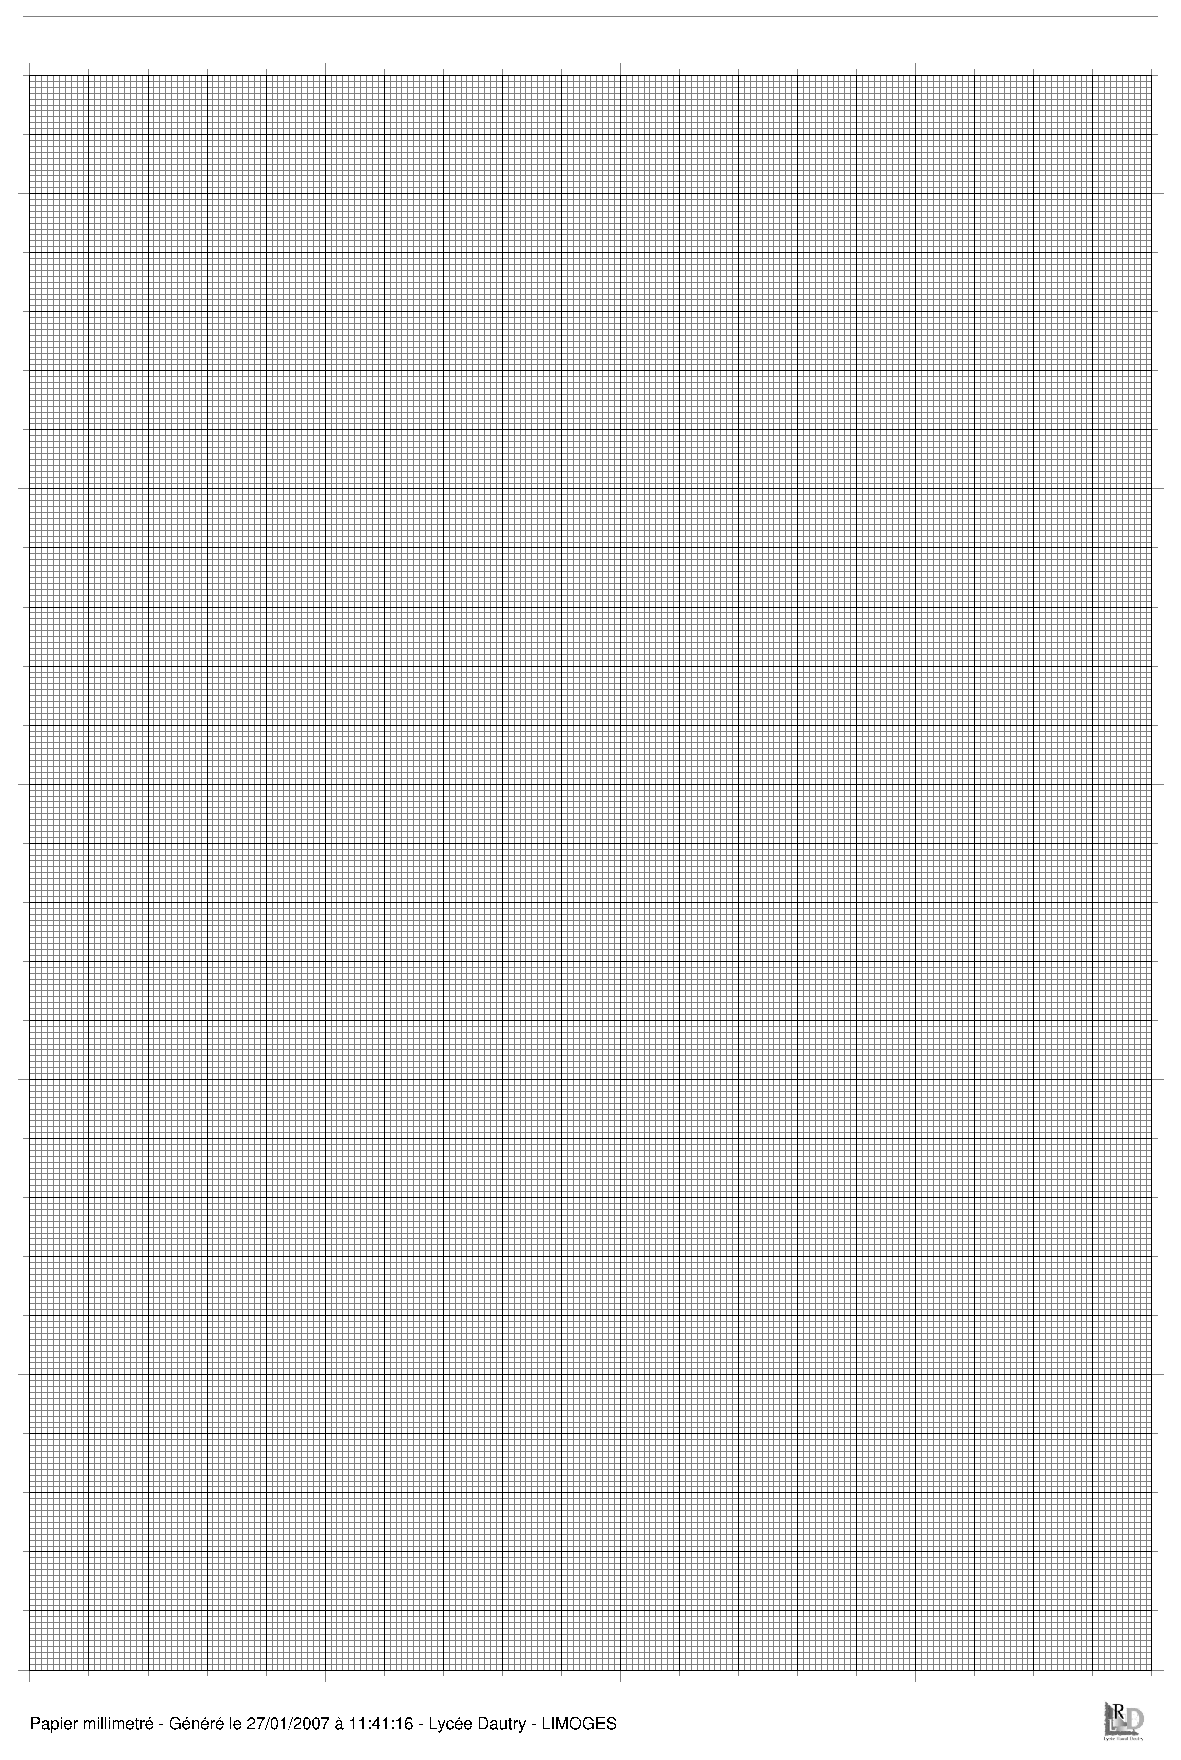
\includegraphics[width=4cm]{papier_milli.eps}
%       &
%       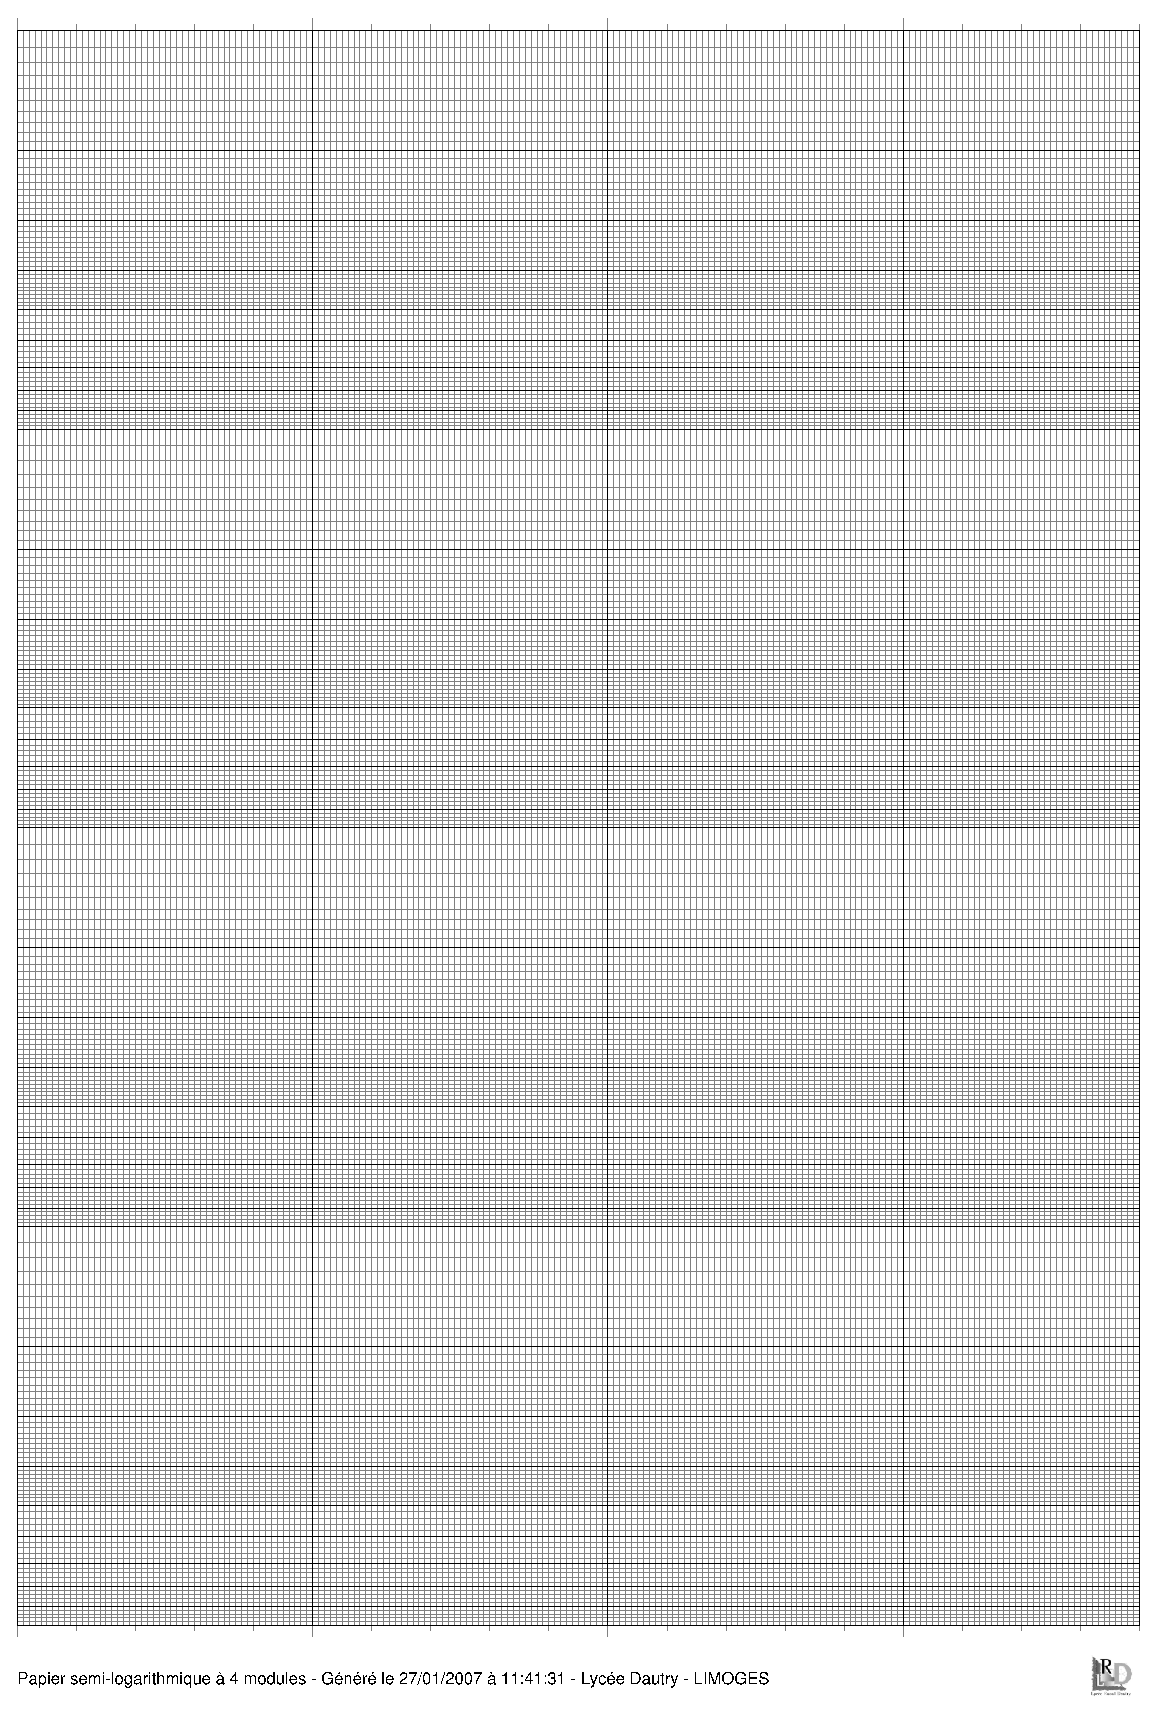
\includegraphics[width=4cm]{papier_semilog4.eps}
%     \end{tabularx}
%   \end{center}

%     %\vressort{1}
% }

\frame{
  \frametitle{Quelques r�alisations (informatique)} 

  \begin{itemize}

  \item Application en ligne de suivi de probl�mes informatiques
 
    \begin{center}
      \url{http://www.celles.net/maintenance}
    \end{center}   

    \begin{itemize}
    \item \'Ecrit en PHP avec connexion � une base de donn�es MySQL
    \end{itemize}

  \begin{center}
    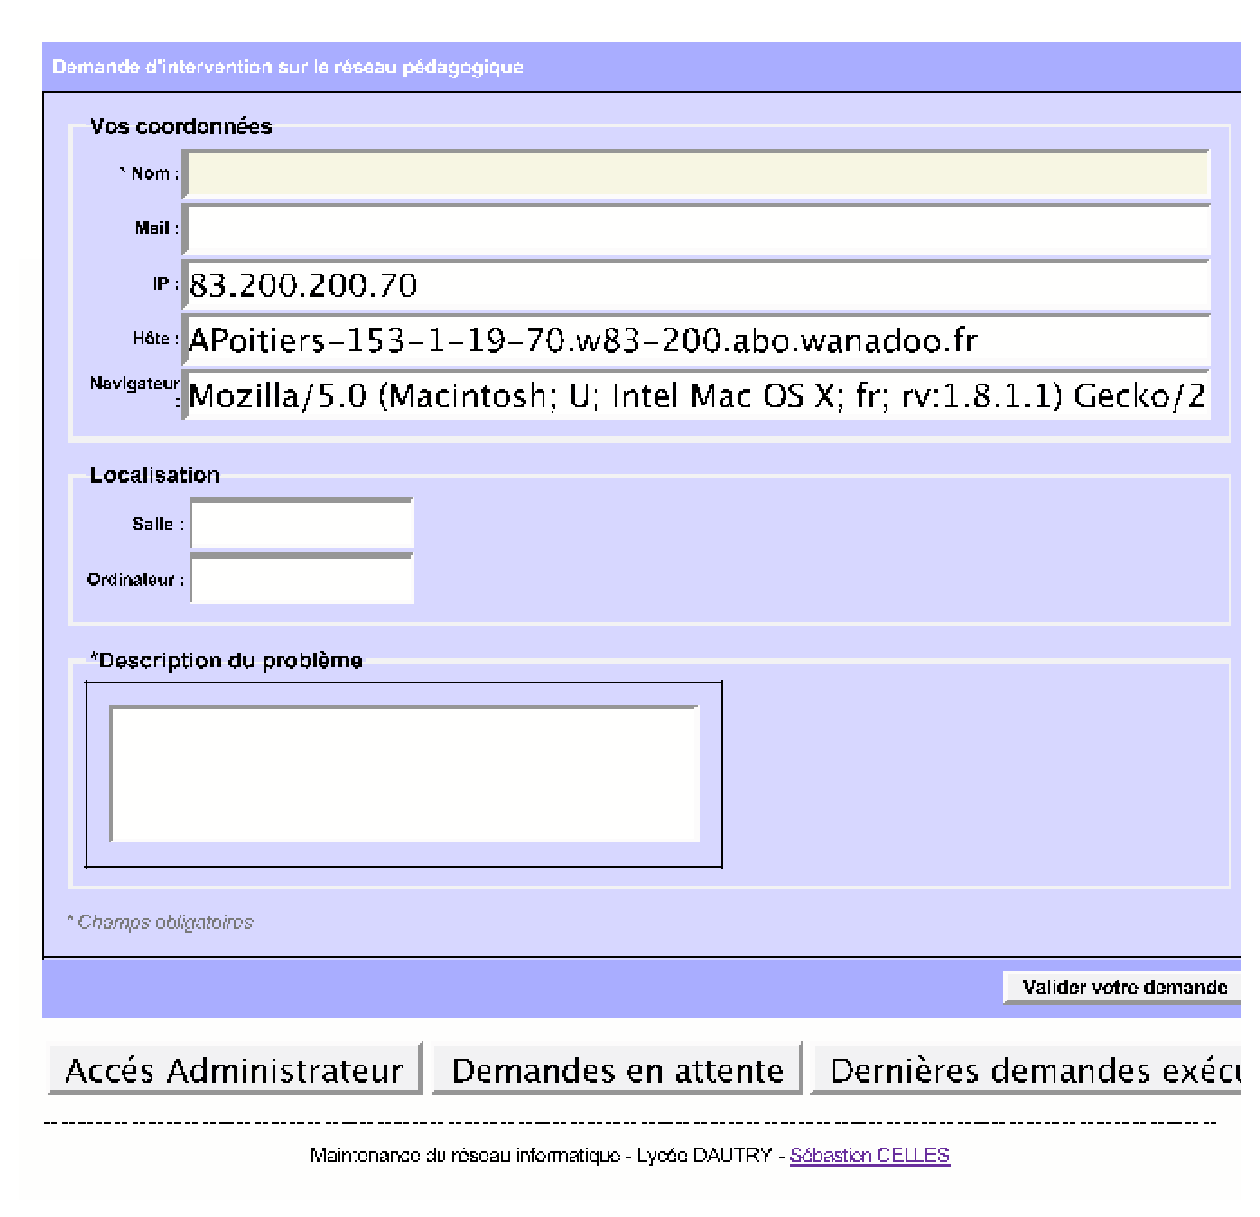
\includegraphics[height=4cm]{maintenance.eps}
  \end{center}


  \end{itemize}
}